\documentclass[border=3pt]{standalone}
% Preâmbulo compartilhado pelos diagramas TikZ da aula 8 de IHR (Métodos de Pesquisa)
\usepackage[T1]{fontenc}
\usepackage[utf8]{inputenc}
\usepackage{lmodern}
\usepackage{amsmath}
\usepackage{xcolor}
\usepackage{tikz}
\usetikzlibrary{arrows.meta,angles,quotes,decorations.pathmorphing,decorations.pathreplacing,calc,
                positioning,shapes.geometric,shapes.misc,backgrounds,fit,
                math}

% Paleta (mesma dos SVGs originais)
% Paleta da disciplina de IHR: acento azul (#1A6FB5), cor de destaque do tema.
% (o nome "dblue" é mantido para não alterar todos os diagramas)
\definecolor{dblue}{HTML}{1A6FB5}
\definecolor{dorange}{HTML}{B3541E}
\definecolor{dgreen}{HTML}{4A7C59}
\definecolor{dred}{HTML}{9C4B4B}
\definecolor{dcream}{HTML}{F4F1EA}
\definecolor{dshade}{HTML}{DDD7C9}

% Função gaussiana (não normalizada por padrão de escala visual)
\pgfmathdeclarefunction{gauss}{3}{%
  \pgfmathparse{1/(#3*sqrt(2*pi))*exp(-((#1-#2)^2)/(2*#3^2))}%
}

% Estilos comuns (prefixo d... para não colidir com chaves internas do pgf)
\tikzset{
  >={Stealth[length=2mm]},
  dguide/.style={gray!55, dashed, line width=0.4pt},
  daxis/.style={gray!60, line width=0.7pt, ->},
  dbody/.style={fill=black!3, draw=black!80, line width=1pt},
  dacc/.style={draw=dblue, line width=1pt},
  dlbl/.style={black!55, font=\small},
  dsub/.style={black!45, font=\footnotesize},
  dstate/.style={circle, draw=black!80, fill=dcream, line width=1pt,
                 minimum size=17mm, font=\large, inner sep=1pt},
  dobs/.style={circle, draw=black!80, fill=dshade, line width=1pt,
               minimum size=14mm, font=\large, inner sep=1pt},
  dbox/.style={rounded corners=2pt, draw=black!80, fill=dcream, line width=1pt,
               align=center, inner sep=6pt},
  dop/.style={circle, draw=black!80, fill=white, line width=1pt,
              minimum size=6mm, inner sep=0pt, font=\small},
  dtrans/.style={->, dblue, line width=1pt},
  dmeas/.style={->, dorange, line width=1pt},
  dcurve/.style={line width=1pt, dblue},
  dcurveb/.style={line width=1.4pt, dorange},
}

\begin{document}
\hyphenpenalty=10000 \exhyphenpenalty=10000 \tolerance=9999 \emergencystretch=3em
\newcommand{\pessm}[4]{% x, y, contorno, preenchimento
  \draw[#3, fill=#4, line width=1.2pt] (#1,#2+0.34) circle (0.22);
  \draw[#3, fill=#4, line width=1.2pt, rounded corners=3pt] (#1-0.38,#2-0.5) rectangle (#1+0.38,#2+0.05);}
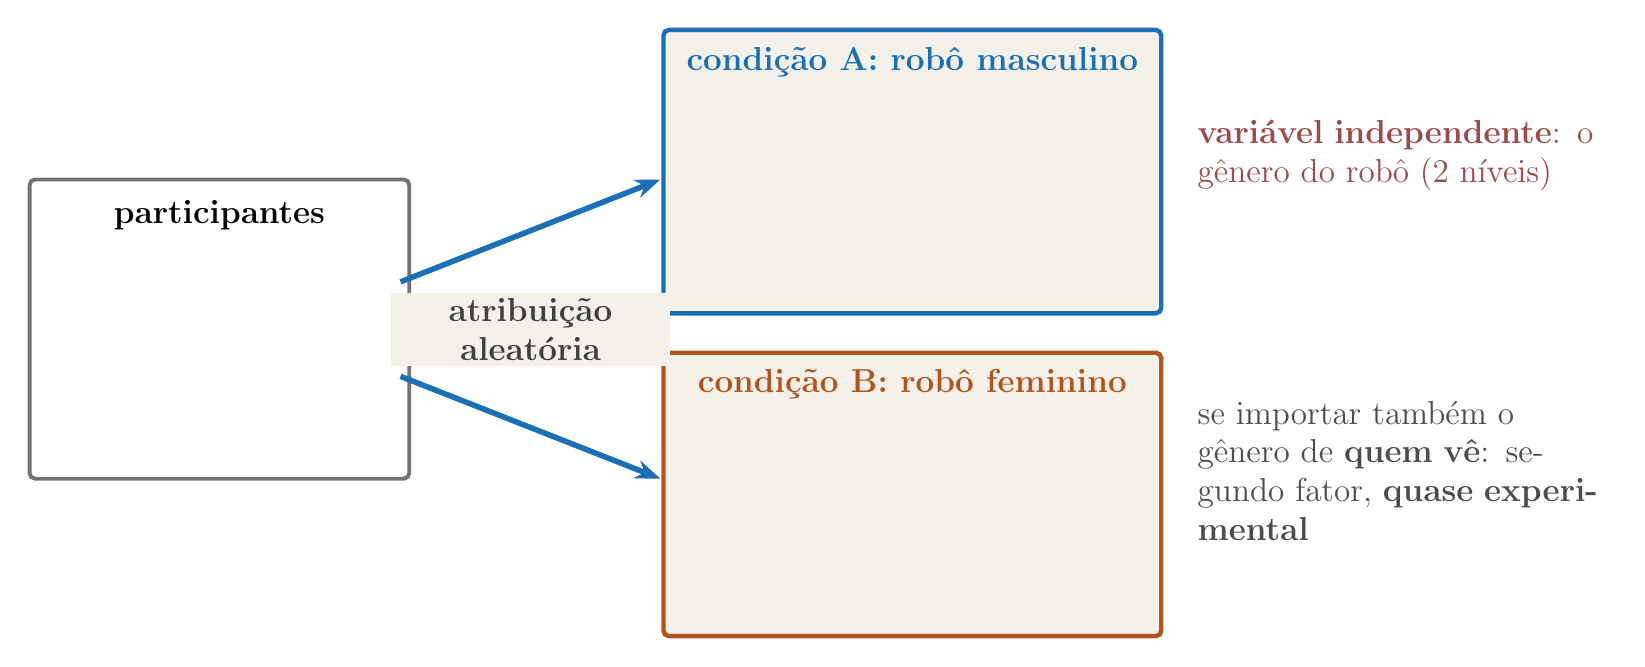
\begin{tikzpicture}[x=1cm,y=1cm]
  \tikzset{g/.style={dbox, text width=5.9cm, minimum height=3.6cm, font=\large, line width=1.6pt, align=center}}
  \node[dbox, draw=black!55, fill=white, line width=1.4pt, text width=4.4cm, minimum height=3.8cm, font=\large, align=center] at (2.4,4.0) {};
  \node[font=\large\bfseries] at (2.4,5.45) {participantes};
  \foreach \x/\y in {1.1/4.5,2.1/4.5,3.1/4.5,1.6/3.2,2.6/3.2,3.6/3.2} {\pessm{\x}{\y}{black!55}{black!8}}
  \node[g, draw=dblue] (a) at (11.2,6.0) {};
  \node[g, draw=dorange] (b) at (11.2,1.9) {};
  \node[font=\large\bfseries, dblue] at (11.2,7.4) {condição A: robô masculino};
  \node[font=\large\bfseries, dorange] at (11.2,3.3) {condição B: robô feminino};
  \foreach \x in {9.5,10.5,11.9,12.9} {\pessm{\x}{5.55}{dblue}{dblue!12}}
  \foreach \x in {9.5,10.5,11.9,12.9} {\pessm{\x}{1.45}{dorange}{dorange!12}}
  \draw[dtrans, line width=2pt, -{Stealth[length=3.2mm]}] (4.7,4.6) -- (8.0,5.9);
  \draw[dtrans, line width=2pt, -{Stealth[length=3.2mm]}] (4.7,3.4) -- (8.0,2.1);
  \node[font=\large\bfseries, black!75, text width=3.4cm, align=center, fill=dcream, inner sep=2pt] at (6.35,4.0) {atribuição\\ aleatória};
  \node[font=\large, dred, anchor=west, text width=5.2cm] at (14.7,6.2) {\textbf{variável independente}: o gênero do robô (2 níveis)};
  \node[font=\large, black!70, anchor=west, text width=5.2cm] at (14.7,2.2) {se importar também o gênero de \textbf{quem vê}: segundo fator, \textbf{quase experimental}};
\end{tikzpicture}
\end{document}
